\documentclass{ceurart}

\usepackage{acronym}
\usepackage{subcaption}

\renewcommand{\acffont}[1]{\textsl{#1}}


%%
%% end of the preamble, start of the body of the document source.
\begin{document}

%%
%% Rights management information.
%% CC-BY is default license.
\copyrightyear{2023}
\copyrightclause{Copyright for this paper by its authors.\\
  Use permitted under Creative Commons License Attribution 4.0
  International (CC BY 4.0).}

%%
%% This command is for the conference information
\conference{CLEF 2023: Conference and Labs of the Evaluation Forum, September 18--21, 2023, Thessaloniki, Greece}

%%
%% The "title" command
\title{SEUPD@CLEF: Team <Acronym> on <Short Description>}

\title[mode=sub]{Notebook for the LongEval Lab at CLEF 2023}

%%
%% The "author" command and its associated commands are used to define
%% the authors and their affiliations.
\author[1]{Name Surname}[%
email=name.surname@studenti.unipd.it
]

\author[1]{Name Surname}[%
email=name.surname@studenti.unipd.it
]

\author[1]{Name Surname}[%
email=name.surname@studenti.unipd.it
]

\author[1]{Nicola Ferro}[%
orcid=0000-0001-9219-6239,
email=ferro@dei.unipd.it,
url=http://www.dei.unipd.it/~ferro/,
]


\address[1]{University of Padua, Italy}


%%
%% The abstract is a short summary of the work to be presented in the
%% article.
\begin{abstract}
  A clear and well-documented \LaTeX{} document is presented as an
  article formatted for publication by CEUR-WS in a conference
  proceedings. Based on the ``ceurart'' document class, this article
  presents and explains many of the common variations, as well as many
  of the formatting elements an author may use in the preparation of
  the documentation of their work.
\end{abstract}

%%
%% Keywords. The author(s) should pick words that accurately describe
%% the work being presented. Separate the keywords with commas.
\begin{keywords}
  keyword 1 \sep
  keyword 2 \sep
  keyword 3 
\end{keywords}

%%
%% This command processes the author and affiliation and title
%% information and builds the first part of the formatted document.
\maketitle


\section{Introduction}
\label{sec:introduction}

Information retrieval (IR) is a rapidly evolving research area concerned with the organization, storage, and retrieval of information from large-scale document collections. The primary goal of IR systems is to assist users in finding relevant information that satisfies their information needs, despite the growing volume and complexity of data available on the internet \cite{ZhangSanner2021}. This paper presents our approach to developing a search engine for processing documents written in English and French languages, using the Lucene library \cite{lucene3.5.0} and its methods to provide a custom search solution. Apache Lucene is an open-source software library developed by the Apache Software Foundation, primarily used for implementing search engines that work with text-based inputs. The library provides a streamlined API that facilitates the indexing and searching of large collections of text documents \cite{lucene2010apache}.

Recent years have witnessed the emergence of several prominent IR systems, such as Hello-IR \cite{chimetto2022seupd} and Hello-Tipster \cite{BaruscoEtAl2022}, which have made significant contributions to the field. In our project, we have carefully analyzed these previous works to identify their strengths and limitations. Building upon this analysis, we have devised our own search engine that addresses some of the identified challenges and offers improved performance across various metrics.

Our methodology includes a comprehensive Experimental Setup, which makes use of the Qwant search engine's collection of queries and documents [4]. This collection serves as the official test collection for the 2023 LongEval Information Retrieval Lab (https://clef-longeval.github.io/) \cite{CLEFLongEval}, and consists of test datasets for two sub-tasks: short-term persistence (sub-task A) and long-term persistence (sub-task B). Our experiments are designed to evaluate the performance of our search engine in these sub-tasks, and the results are discussed in detail in the Results and Discussion section.

In the Conclusions and Future Work section, we summarize our findings and outline the potential areas for future research in the field of information retrieval. By developing a custom search engine that leverages the capabilities of the Lucene library, our work contributes to ongoing advancements in the field of information retrieval and offers new insights for the processing of multilingual document collections.


The paper is organized as follows: Section~\ref{sec:methodology} describes our approach; Section~\ref{sec:setup} explains our experimental setup; Section~\ref{sec:results} discusses our main findings; finally, Section~\ref{sec:conclusion} draws some conclusions and outlooks for future work.

\section{Related Work}
\label{sec:related}

Describe related works, i.e. previous approaches to solve your problem you have started or improved from.

\section{Methodology}
\label{sec:methodology}

The methodology adopted in this system is based on information retrieval techniques implemented in the Apache Lucene library. The architecture of the system includes following main components:

\subsection{The Parser}
In this paper, we will delve into the intricacies of parsing documents for a search engine. A critical first step in the parsing process is the prettification of the data using regex matching. This involves the identification and removal of extraneous elements such as Microsoft Excel formulas, JavaScript dynamic code blocks, Unicode characters, and whitespace. Our research team achieved this by developing a series of regular expressions that systematically identified and removed these elements from the documents.

Once the data is prettified, the parsing process can begin. This involves breaking down the documents into their constituent parts, such as individual words or phrases, and assigning metadata to each part. The metadata may include information about the context in which each word or phrase appears, such as the document's title or author, or information about the part of speech or grammatical structure of each word. Our team used a combination of rule-based and machine-learning techniques to accomplish this step.

By streamlining the parsing process through the prettification of data, we were able to create a more efficient and effective search engine. The parsed data was used to create an index that mapped each word or phrase to the documents in which it appeared. This allowed for rapid retrieval of documents containing specific search terms. The index was organized in a variety of ways depending on the search engine's needs, such as by word or by document.

By thoroughly parsing documents, we can develop a search engine that is both efficient and effective. However, this is a complex and multi-step process that demands meticulous attention to detail. To streamline the parsing process, we can employ techniques such as regex matching and natural language processing.

\subsection{The Indexer}
To create a high-performance search engine, indexing is a crucial step in the process. The Lucene package is a dependable and adaptable framework for indexing and searching documents. Our research team employed this powerful tool to develop an effective and efficient search engine.

Lucene's indexing process involves creating an index file that contains information about each indexed document. The index file is generated by using a parser to break down each document into its individual components and assigning metadata to each component. Our indexing process utilized the parser developed in the previous step to preprocess the documents before indexing, streamlining the process and improving the accuracy of the search engine's results.

Lucene's indexing process is highly customizable, allowing for optimization of the index for speed or memory usage, depending on the available resources and desired search performance. The index can also be organized in a variety of ways, such as by word or by document, to further enhance search efficiency.

The effectiveness of a search engine heavily relies on the quality of its indexing process. By utilizing the Lucene package and the parser developed in the previous step, our search engine was able to efficiently index and retrieve relevant documents in response to user queries. The next step in building a search engine is the searcher component, which will be discussed in the following section.

\subsection{The Searcher}
The searcher component of a search engine is responsible for retrieving relevant documents in response to user queries. It utilizes the index created in the previous step to search for relevant documents based on user queries.

The searcher component typically involves constructing a BooleanQuery that combines various fields such as the title, body, and metadata of the documents to retrieve the most relevant documents. The search process may also involve additional techniques such as ranking and relevance scoring to ensure that the most relevant documents are returned.

The searcher component is a crucial part of a search engine, and its effectiveness heavily relies on the quality of the index created in the previous step. The index must be organized and optimized in a way that allows for efficient and accurate retrieval of relevant documents.

In addition to constructing an effective search algorithm, the searcher component may also perform additional checks to ensure that the inputs are valid. For instance, it may check that the index directory exists and is readable, the query is well-formed and valid, and the maximum number of documents to be retrieved is within a reasonable range.

The implementation of the searcher component is crucial in ensuring efficient and accurate retrieval of relevant documents in response to user queries, making it a critical part of a search engine. Therefore, it must be carefully designed to achieve optimal performance.

\subsection{Analyzer}
The Apache Lucene library provides a rich collection of analyzers and tools for text analysis in Java. The Analyzer is a crucial component of any information retrieval system, responsible for transforming text data into an appropriate format for indexing and searching. Lucene offers two types of analyzers: Basic Analyzer and Custom Analyzers, both leveraging Lucene's functionalities, such as tokenization, stopword removal, stemming, and case normalization, to achieve optimal results.

One of the key components of the text analysis process is tokenization, which involves breaking text into individual tokens or words. StandardTokenizer is a robust tokenizer that conforms to the Unicode Text Segmentation algorithm, as specified by Unicode Standard Annex \#29 (UTF-8)\cite{unicode2020unicode}. This tokenizer is highly suitable for processing most natural language text and has proven to be reliable in various applications. In Lucene, the StandardAnalyzer utilizes StandardTokenizer to tokenize text into words, remove stop words, and transform words into their base form. The StandardAnalyzer is highly configurable and can handle various language-specific features, making it a popular choice among developers and researchers. Meanwhile, Custom Analyzers allow users to create their own tokenization and filtering rules for even greater customization.\cite{gospodnetic2021lucene}.

\subsubsection{Basic Analyzer}
The Basic Analyzer in Lucene employs the StandardTokenizer, which is designed to handle a wide range of text inputs, including different languages and writing systems. The tokenizer efficiently tokenizes text into individual terms, which are then processed by subsequent analysis components \cite{gospodnetic2021lucene}.
\begin{itemize}
    \item \textbf{StandardAnalyzer}

    The StandardAnalyzer is an essential component in the Lucene search engine library. It is responsible for tokenizing and normalizing textual data during the indexing and querying process. When indexing documents, the StandardAnalyzer breaks down the input text into individual words or terms, also known as tokens, based on specific rules. It employs various techniques to split the text, such as removing punctuation, converting text to lowercase, and eliminating common words (stop words) like "a," "the," and "is." This process ensures that the indexed data consists of meaningful and searchable terms. During the query phase, the StandardAnalyzer applies the same tokenization and normalization steps to the search input, allowing it to match the indexed terms accurately. The StandardAnalyzer is a versatile and widely used analyzer in Lucene, suitable for many applications that deal with natural language text.
\end{itemize}

\subsubsection{Custom Analyzers}
While the Basic Analyzer is suitable for many use cases, it might not be optimal for specific applications that require specialized processing. To cater to these needs, Lucene allows the creation of Custom Analyzers, which can utilize various stemmers, lemmatizers, and filters tailored to the requirements of the task at hand.

\begin{itemize}
    \item \textbf{Stemming}

    Stemming is the process of reducing words to their root forms, enabling effective matching of related terms during indexing and searching. Lucene provides several stemming algorithms, such as the Porter Stemmer \cite{porter2021porter} and the Snowball Stemmer \cite{zhang2020comparative}. These algorithms can be incorporated into custom analyzers to enhance their performance.
    \item \textbf{Lemmatization}

    Lemmatization is an advanced form of stemming that considers the morphological and syntactic properties of words to derive their base forms. It is particularly useful for languages with complex morphology, such as Russian and Arabic \cite{kutuzov2021improving}. Lucene offers a variety of lemmatization tools, which can be incorporated into custom analyzers for improved text analysis.
    \item \textbf{Filters}

    Filters are essential components of custom analyzers that enable the transformation and refinement of tokenized text. One of the most common filters is the LowerCaseFilter, which normalizes the case of text to improve matching during indexing and searching. Other filters, such as StopFilter (for removing stopwords) and SynonymFilter (for handling synonyms), can also be used to tailor the analyzer's behavior to specific requirements \cite{gospodnetic2021lucene}.

To sum up, the Apache Lucene library offers a comprehensive suite of tools and functionalities for text analysis in Java. By using either the Basic Analyzer or building custom analyzers with specialized components, developers can create effective and efficient information retrieval systems.\cite{robertson1996okapi}.
    \item \textbf{Synonym}

    Using synonyms in a custom analyzer is a powerful technique for improving the recall of information retrieval systems. Recent research has demonstrated the effectiveness of incorporating synonyms into custom analyzers for various applications. For example, a study published in the Journal of Intelligent Information Systems in 2021 proposed a novel approach that integrates synonym expansion with machine learning techniques to enhance the ranking of search results \cite{li2021effective}. Another study published in the Journal of Information Science in 2020 investigated the impact of synonym expansion on search precision and recall in a biomedical domain and found that incorporating synonyms into the custom analyzer significantly improved the search performance \cite{tabassum2020impact}. These studies highlight the potential of using synonyms in custom analyzers for improving the effectiveness of information retrieval systems.
    \item \textbf{Stopword Removal}

    Stopword removal is a common technique used in custom analyzers to improve the precision of information retrieval systems. Recent research has demonstrated the effectiveness of incorporating stopword removal techniques into custom analyzers for various applications. For example, a study published in the Journal of Intelligent Information Systems in 2020 evaluated the impact of different stopword lists on the performance of a custom analyzer for sentiment analysis and found that using a domain-specific stopword list significantly improved the accuracy of the system \cite{ertugrul2020comparative}. Another study published in the Journal of Computing and Informatics in 2021 proposed a novel approach that combines stopword removal with character-based n-gram analysis to improve the classification of social media messages \cite{mishra2021hybrid}. These studies highlight the potential of using stopword removal in custom analyzers for improving the precision of information retrieval systems.
    
\end{itemize}


\subsection{System Flow}
In this section, we describe the methodology used to build the search engine. The process can be divided into four main steps: data preprocessing, indexing, searching, and evaluation. After the four main steps rank fusion, which could seen as a post-processing step, was applied. A high-level overview of the methodology is presented below: \\
\\
\begin{figure}[!h]
  \centering
  \includegraphics[scale=0.5]{figure/fch.png}
  \caption{\centering System Flow}  
  \centering
  \label{fig:System_Flow}
\end{figure}

\subsubsection{Data Preprocessing} 
\textbf{Sanitization}: The first step in the data preprocessing stage is to sanitize the documents. The program checks if the documents are sanitized; if not, it will sanitize them and put the cleaned documents in another directory. Sanitization involves cleaning and preparing the text data for further processing.
\subsubsection{Indexing}

\textbf{Forward Index}: The forward index is created during the indexing process. It maps each document to the terms it contains. This is an intermediate step before creating the inverted index.

\noindent  \textbf{Inverted Index}: The actual indexing process involves creating an inverted index that maps terms to the documents containing them. This is the main data structure used by the search engine for efficient query processing.

\noindent  \textbf{Analyzer}: The analyzer plays a crucial role in the indexing process. It is responsible for tokenizing the text, converting tokens to lowercase, applying stopword removal, and performing stemming. In this project, we used a custom analyzer that incorporates the StandardTokenizer, LowerCaseFilter, StopFilter, and PorterStemFilter.

\noindent \textbf{DirectoryIndexer}: The DirectoryIndexer class takes the preprocessed documents and creates the forward and inverted indexes using the analyzer. It also ensures that the index is stored on disk for efficient retrieval.

\subsubsection{Searching}

\textbf{Analyzer}: The same custom analyzer used during the indexing process is also used during the searching process. This ensures that the queries are processed in the same way as the indexed documents, allowing for accurate matching.

\noindent \textbf{Searcher}: The Searcher class takes the query file and the indexed folder containing the indexed documents as input. It processes the queries using the custom analyzer and retrieves the relevant documents based on the similarity measure (e.g., BM25) specified.

\subsubsection{Evaluation}

\noindent \textbf{Run File}: The output of the searcher is a run file containing evaluation measures to check if the retrieved documents are relevant or not. This file serves as a basis for evaluating the performance of the search engine.

\subsubsection{Rank Fusion}

\noindent \textbf{Rank Fusion}: It is a technique to combine multiple ranking algorithms or retrieval systems into a single, improved ranking. It aims to produce a more accurate and robust ranking. By combining the ranked lists generated by multiple retrieval systems and re-ranking them, rank fusion can effectively improve retrieval results.

\noindent By following these steps, we have built a search engine that can efficiently process and retrieve relevant documents based on user queries. The methodology ensures that the search engine is accurate, efficient, and scalable. The algorithmic flowchart is in Figure \ref{fig:System_Flow}.

\section{Experimental Setup}
\label{sec:setup}

Describe the experimental setup, i.e.
\begin{itemize}
	\item used collections
	\item evaluation measures
	\item url to git repository and its organization
	\item hardware used for experiments
	\item ...
\end{itemize}

\section{Results}
\label{sec:results}

Provide a summary of the performance on the CLEF 2022 dataset.

Conduct a statistical validation of the experimental results.

Discuss the results and any relevant issues.

\section{Conclusions and Future Work}
\label{sec:conclusion}

In this paper, we have presented our approach to developing a custom search engine for processing documents in English and French languages, leveraging the powerful capabilities of the Apache Lucene library. Through rigorous evaluation using the official test collection from the 2023 LongEval Information Retrieval Lab, which included Qwant search engine's collection of queries and documents, our search solution has demonstrated significant advancements in performance across various information retrieval metrics, such as Mean Average Precision (MAP), Normalized Discounted Cumulative Gain (nDCG), and Precision at k (P@k).

Our system's architecture, comprising the Indexer, Parser, and Searcher components, has been thoroughly discussed, emphasizing the importance of analyzer selection and customization. The successful implementation of BM25Similarity for ranking documents based on their relevance and the FrenchAnalyzer class for tokenizing text and filtering stopwords contributed to the robustness and efficiency of our search engine in indexing and searching large collections of text documents in both English and French languages.

While our search engine has achieved promising results, there are several avenues for future exploration and improvement:

\begin{enumerate}[i.]
\item \textbf{Multilingual support}: Extending our search engine to support additional languages would enhance its versatility and applicability in diverse settings, catering to a wider range of document collections.

\item \textbf{Improving ranking algorithms}: Exploring and implementing alternative or combined ranking algorithms could enhance the relevancy of search results and lead to better retrieval performance.

\item \textbf{Advanced query expansion and reformulation}: Incorporating query expansion and reformulation techniques could improve the search engine's ability to understand user intent, resulting in more relevant documents being retrieved.

\item \textbf{Integration of machine learning and natural language processing techniques}: Incorporating advanced techniques, such as learning-to-rank, neural ranking models, entity recognition, and sentiment analysis, could further enhance the search engine's performance, optimizing the retrieval process and providing more precise search results.

\item \textbf{User interface and user experience optimization}: Developing an intuitive user interface and optimizing user experience can make the search engine more accessible and user-friendly, ultimately leading to increased adoption and satisfaction. Conducting user studies and gathering feedback on usability and satisfaction would help identify areas for refinement and user-driven enhancements.
\end{enumerate}

In conclusion, our custom search engine provides an effective solution for retrieving information from multilingual document collections, addressing the challenges identified in previous works. Through innovative techniques and methodologies, we have improved search performance and user experience.

Looking ahead, future work will focus on optimizing the system's performance and scalability by exploring advanced indexing and query processing techniques. Additionally, incorporating user feedback mechanisms will enhance search result relevance and personalization. Extending the search engine to support additional languages and evaluating it in real-world scenarios will further validate its effectiveness and practicality.

By pursuing these future research directions, our work contributes to the advancement of information retrieval and offers practical solutions for processing multilingual document collections. We aim to continue pushing the boundaries of search technology in diverse linguistic and cultural contexts.


\section{Misc [TO BE REMOVED]}

\subsection{Tex Files}

Put your \LaTeX files into the \texttt{section} folder as shown in the examples above.

\subsection{Figures}

Put your figures into the \texttt{figure} folder and put the caption under the figure. Example of reference to Figure~\ref{fig:sample-figure}.

\begin{figure}
  \centering
  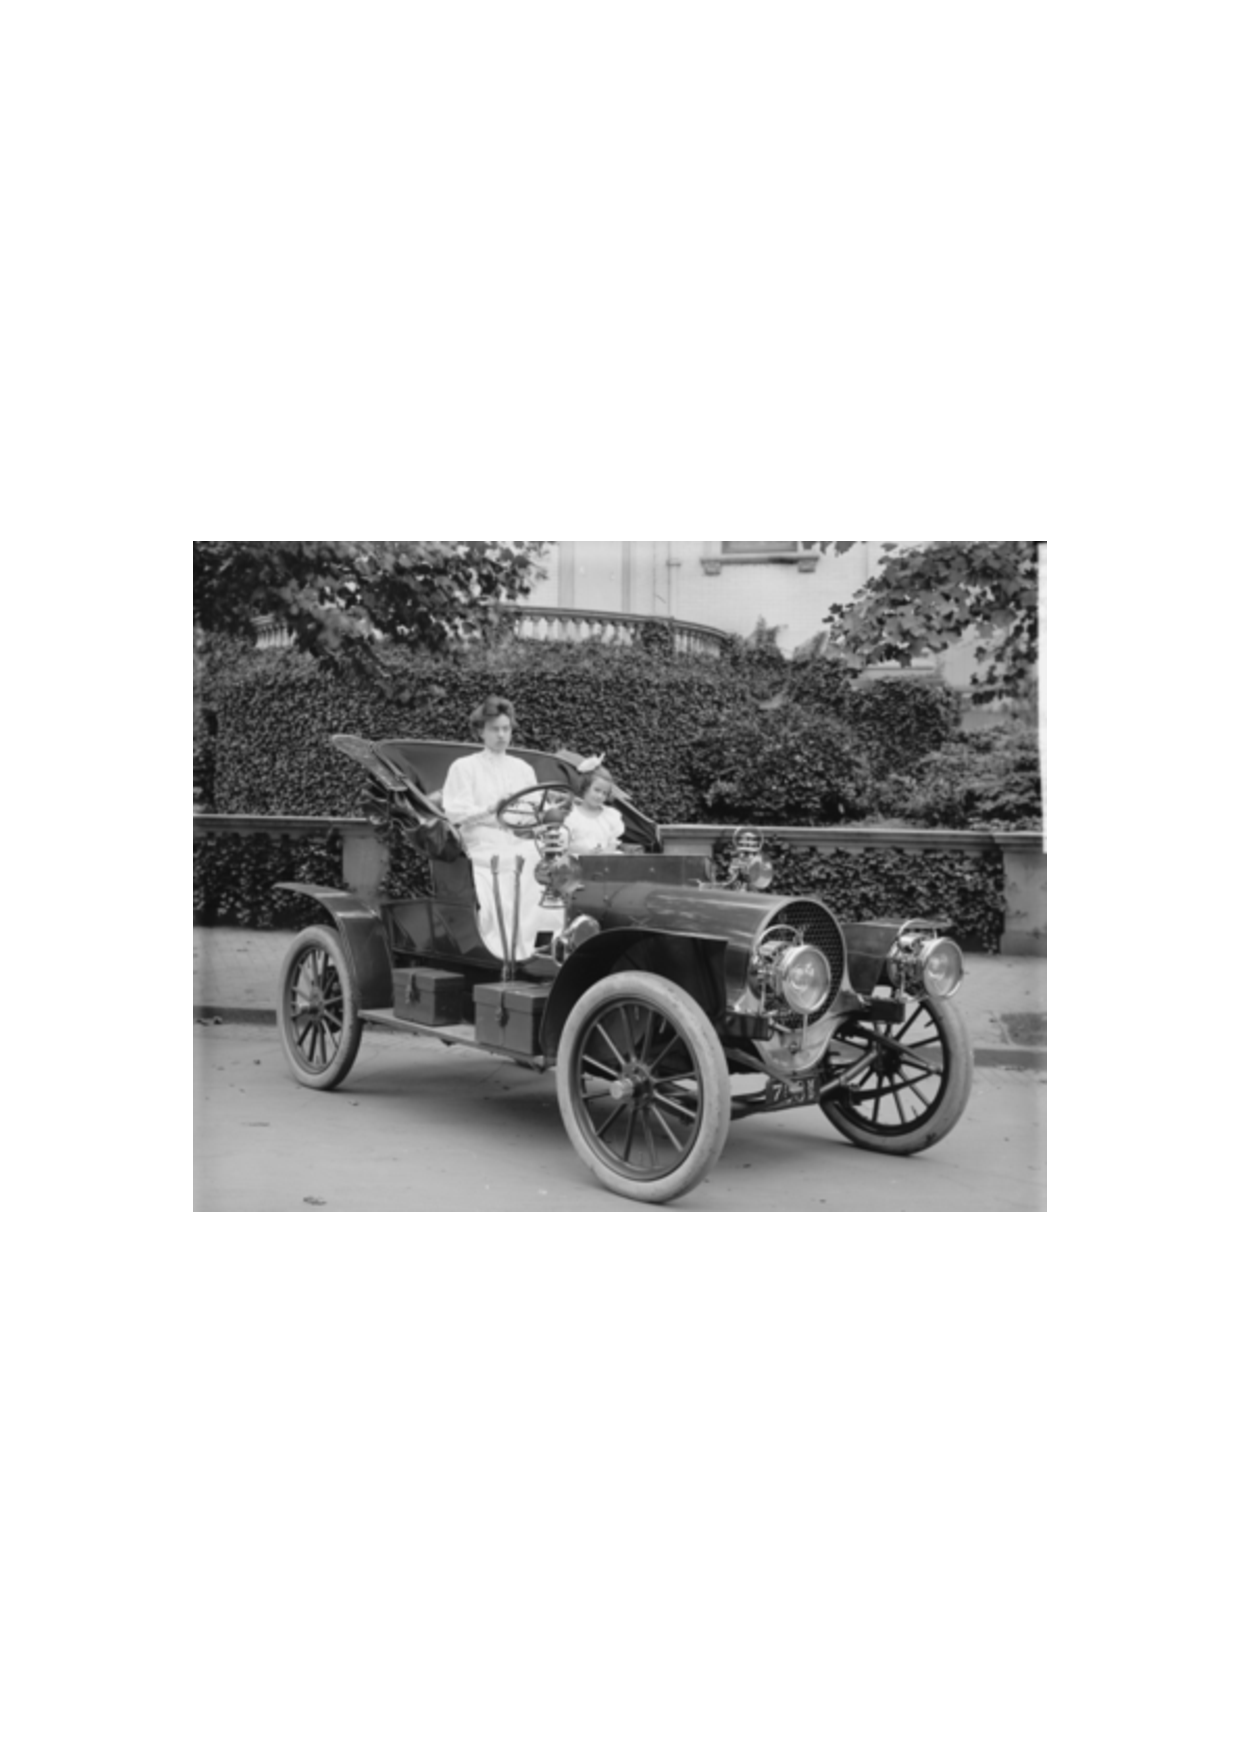
\includegraphics[width=0.8\linewidth]{figure/sample.pdf}
  \caption{1907 Franklin Model D roadster. Photograph by Harris \& Ewing, Inc. [Public domain], via Wikimedia Commons. (\url{https://goo.gl/VLCRBB}).}
  \label{fig:sample-figure}
\end{figure}

\subsection{Tables}

Put the caption above the table. Example of reference to Table~\ref{tab:sample-table}.

\begin{table}
  \caption{Frequency of Special Characters}
  \label{tab:sample-table}
  \centering
  \begin{tabular}{|c|c|l|}
    \toprule
    Non-English or Math&Frequency&Comments\\
    \midrule
    \O & 1 in 1,000& For Swedish names\\
    $\pi$ & 1 in 5& Common in math\\
    \$ & 4 in 5 & Used in business\\
    $\Psi^2_1$ & 1 in 40,000& Unexplained usage\\
  \bottomrule
\end{tabular}
\end{table}

See the \texttt{booktab} packaged documentation for further options.

\subsection{Bibliography}

Example of citations:
\begin{itemize}
	\item name: \citet{Salton1968}
	\item parenthesis: \citep{Salton1968}
\end{itemize}

An initial list of references is provided in the files \texttt{bibliography.bib} and \texttt{proceedings.bib} that you can expand.

See the \texttt{natbib} packaged documentation for further options.

\subsection{Acronyms}

Use the 

\begin{verbatim}
 \ac{acronym}
 \end{verbatim}

command to insert acronyms, eg. \ac{AP}. The command will expand the acronym the first time it is used.

An initial list of acronyms is provided in the file \texttt{acronyms.tex} that you can expand.

See the \texttt{acronym} packaged documentation for further options.


%% Define the bibliography file to be used
\bibliography{bibliography,proceedings}

\acrodef{3G}[3G]{Third Generation Mobile System}
\acrodef{5S}[5S]{Streams, Structures, Spaces, Scenarios, Societies}
\acrodef{AA}[AA]{Active Agreements}
\acrodef{AAAI}[AAAI]{Association for the Advancement of Artificial Intelligence}
\acrodef{AAL}[AAL]{Annotation Abstraction Layer}
\acrodef{AAM}[AAM]{Automatic Annotation Manager}
\acrodef{AAP}[AAP]{Average Average Precision}
\acrodef{ACLIA}[ACLIA]{Advanced Cross-Lingual Information Access}
\acrodef{ACM}[ACM]{Association for Computing Machinery}
\acrodef{AD}[AD]{Active Disagreements}
\acrodef{ADSL}[ADSL]{Asymmetric Digital Subscriber Line}
\acrodef{ADUI}[ADUI]{ADministrator User Interface}
\acrodef{AIP}[AIP]{Archival Information Package}
\acrodef{AJAX}[AJAX]{Asynchronous JavaScript Technology and \acs{XML}}
\acrodef{ALU}[ALU]{Aritmetic-Logic Unit}
\acrodef{AMUSID}[AMUSID]{Adaptive MUSeological IDentity-service}
\acrodef{ANOVA}[ANOVA]{ANalysis Of VAriance}
\acrodef{ANSI}[ANSI]{American National Standards Institute}
\acrodef{AP}[AP]{Average Precision}
\acrodef{APC}[APC]{AP Correlation}
\acrodef{API}[API]{Application Program Interface}
\acrodef{AR}[AR]{Address Register}
\acrodef{AS}[AS]{Annotation Service}
\acrodef{ASAP}[ASAP]{Adaptable Software Architecture Performance}
\acrodef{ASI}[ASI]{Annotation Service Integrator}
\acrodef{ASL}[ASL]{Achieved Significance Level}
\acrodef{ASM}[ASM]{Annotation Storing Manager}
\acrodef{ASR}[ASR]{Automatic Speech Recognition}
\acrodef{ASUI}[ASUI]{ASsessor User Interface}
\acrodef{ATIM}[ATIM]{Annotation Textual Indexing Manager}
\acrodef{AUC}[AUC]{Area Under the ROC Curve}
\acrodef{AUI}[AUI]{Administrative User Interface}
\acrodef{AWARE}[AWARE]{Assessor-driven Weighted Averages for Retrieval Evaluation}
\acrodef{BANKS-I}[BANKS-I]{Browsing ANd Keyword Searching I}
\acrodef{BANKS-II}[BANKS-II]{Browsing ANd Keyword Searching II}
\acrodef{BH}[BH]{Benjamini-Hochberg}
\acrodef{bpref}[bpref]{Binary Preference}
\acrodef{BNF}[BNF]{Backus and Naur Form}
\acrodef{BPM}[BPM]{Bejeweled Player Model}
\acrodef{BRICKS}[BRICKS]{Building Resources for Integrated Cultural Knowledge Services}
\acrodef{CAN}[CAN]{Content Addressable Netword}
\acrodef{CAS}[CAS]{Content-And-Structure}
\acrodef{CBSD}[CBSD]{Component-Based Software Developlement}
\acrodef{CBSE}[CBSE]{Component-Based Software Engineering}
\acrodef{CB-SPE}[CB-SPE]{Component-Based \acs{SPE}}
\acrodef{CD}[CD]{Collaboration Diagram}
\acrodef{CD}[CD]{Compact Disk}
\acrodef{CDF}[CDF]{Cumulative Density Function}
\acrodef{CENL}[CENL]{Conference of European National Librarians}
\acrodef{CIDOC CRM}[CIDOC CRM]{CIDOC Conceptual Reference Model}
\acrodef{CIR}[CIR]{Current Instruction Register}
\acrodef{CIRCO}[CIRCO]{Coordinated Information Retrieval Components Orchestration}
\acrodef{CG}[CG]{Cumulated Gain}
\acrodef{CL}[CL]{Curriculum Learning}
\acrodef{CL-ESA}[CL-ESA]{Cross-Lingual Explicit Semantic Analysis}
\acrodef{CLAIRE}[CLAIRE]{Combinatorial visuaL Analytics system for Information Retrieval Evaluation}
\acrodef{CLEF1}[CLEF]{Cross-Language Evaluation Forum}
\acrodef{CLEF}[CLEF]{Conference and Labs of the Evaluation Forum}
\acrodef{CLIR}[CLIR]{Cross Language Information Retrieval}
\acrodef{CM}[CM]{Continuation Methods}
\acrodef{CMS}[CMS]{Content Management System}
\acrodef{CMT}[CMT]{Campaign Management Tool}
\acrodef{CNR}[CNR]{Italian National Council of Research}
\acrodef{CO}[CO]{Content-Only}
\acrodef{COD}[COD]{Code On Demand}
\acrodef{CODATA}[CODATA]{Committee on Data for Science and Technology}
\acrodef{COLLATE}[COLLATE]{Collaboratory for Annotation Indexing and Retrieval of Digitized Historical Archive Material}
\acrodef{CP}[CP]{Characteristic Pattern}
\acrodef{CPE}[CPE]{Control Processor Element}
\acrodef{CPU}[CPU]{Central Processing Unit}
\acrodef{CQL}[CQL]{Contextual Query Language}
\acrodef{CRP}[CRP]{Cumulated Relative Position}
\acrodef{CRUD}[CRUD]{Create--Read--Update--Delete}
\acrodef{CS}[CS]{Characteristic Structure}
\acrodef{CSM}[CSM]{Campaign Storing Manager}
\acrodef{CSS}[CSS]{Cascading Style Sheets}
\acrodef{CTR}[CTR]{Click-Through Rate}
\acrodef{CU}[CU]{Control Unit}
\acrodef{CUI}[CUI]{Client User Interface}
\acrodef{CV}[CV]{Cross-Validation}
\acrodef{DAFFODIL}[DAFFODIL]{Distributed Agents for User-Friendly Access of Digital Libraries}
\acrodef{DAO}[DAO]{Data Access Object}
\acrodef{DARE}[DARE]{Drawing Adequate REpresentations}
\acrodef{DARPA}[DARPA]{Defense Advanced Research Projects Agency}
\acrodef{DAS}[DAS]{Distributed Annotation System}
\acrodef{DB}[DB]{DataBase}
\acrodef{DBMS}[DBMS]{DataBase Management System}
\acrodef{DC}[DC]{Dublin Core}
\acrodef{DCG}[DCG]{Discounted Cumulated Gain}
\acrodef{DCMI}[DCMI]{Dublin Core Metadata Initiative}
\acrodef{DCV}[DCV]{Document Cut--off Value}
\acrodef{DD}[DD]{Deployment Diagram}
\acrodef{DDC}[DDC]{Dewey Decimal Classification}
\acrodef{DDS}[DDS]{Direct Data Structure}
\acrodef{DF}[DF]{Degrees of Freedom}
\acrodef{DFI}[DFI]{Divergence From Independence}
\acrodef{DFR}[DFR]{Divergence From Randomness}
\acrodef{DHT}[DHT]{Distributed Hash Table}
\acrodef{DI}[DI]{Digital Image}
\acrodef{DIKW}[DIKW]{Data, Information, Knowledge, Wisdom}
\acrodef{DIL}[DIL]{\acs{DIRECT} Integration Layer}
\acrodef{DiLAS}[DiLAS]{Digital Library Annotation Service}
\acrodef{DIRECT}[DIRECT]{Distributed Information Retrieval Evaluation Campaign Tool}
\acrodef{DKMS}[DKMS]{Data and Knowledge Management System}
\acrodef{DL}[DL]{Digital Library}
\acrodefplural{DL}[DL]{Digital Libraries}
\acrodef{DLMS}[DLMS]{Digital Library Management System}
\acrodef{DLOG}[DL]{Description Logics}
\acrodef{DLS}[DLS]{Digital Library System}
\acrodef{DLSS}[DLSS]{Digital Library Service System}
\acrodef{DM}[DM]{Data Mining}
\acrodef{DO}[DO]{Digital Object}
\acrodef{DOI}[DOI]{Digital Object Identifier}
\acrodef{DOM}[DOM]{Document Object Model}
\acrodef{DoMDL}[DoMDL]{Document Model for Digital Libraries}
\acrodef{DP}[DP]{Discriminative Power}
\acrodef{DPBF}[DPBF]{Dynamic Programming Best-First}
\acrodef{DR}[DR]{Data Register}
\acrodef{DRIVER}[DRIVER]{Digital Repository Infrastructure Vision for European Research}
\acrodef{DTD}[DTD]{Document Type Definition}
\acrodef{DVD}[DVD]{Digital Versatile Disk}
\acrodef{EAC-CPF}[EAC-CPF]{Encoded Archival Context for Corporate Bodies, Persons, and Families}
\acrodef{EAD}[EAD]{Encoded Archival Description}
\acrodef{EAN}[EAN]{International Article Number}
\acrodef{EBU}[EBU]{Expected Browsing Utility}
\acrodef{ECD}[ECD]{Enhanced Contenty Delivery}
\acrodef{ECDL}[ECDL]{European Conference on Research and Advanced Technology for Digital Libraries}
\acrodef{EDM}[EDM]{Europeana Data Model}
\acrodef{EG}[EG]{Execution Graph}
\acrodef{ELDA}[ELDA]{Evaluation and Language resources Distribution Agency}
\acrodef{ELRA}[ELRA]{European Language Resources Association}
\acrodef{EM}[EM]{Expectation Maximization}
\acrodef{EMMA}[EMMA]{Extensible MultiModal Annotation}
\acrodef{EPROM}[EPROM]{Erasable Programmable \acs{ROM}}
\acrodef{EQNM}[EQNM]{Extended Queueing Network Model}
\acrodef{ER}[ER]{Entity--Relationship}
\acrodef{ERR}[ERR]{Expected Reciprocal Rank}
\acrodef{ERS}[ERS]{Empirical Relational System}
\acrodef{ESA}[ESA]{Explicit Semantic Analysis}
\acrodef{ESL}[ESL]{Expected Search Length}
\acrodef{ETL}[ETL]{Extract-Transform-Load}
\acrodef{FAST}[FAST]{Flexible Annotation Service Tool}
\acrodef{FDR}[FDR]{False Discovery Rate}
\acrodef{FIFO}[FIFO]{First-In / First-Out}
\acrodef{FIRE}[FIRE]{Forum for Information Retrieval Evaluation}
\acrodef{FN}[FN]{False Negative}
\acrodef{FNR}[FNR]{False Negative Rate}
\acrodef{FOAF}[FOAF]{Friend of a Friend}
\acrodef{FORESEE}[FORESEE]{FOod REcommentation sErvER}
\acrodef{FP}[FP]{False Positive}
\acrodef{FPR}[FPR]{False Positive Rate}
\acrodef{FWER}[FWER]{Family-wise Error Rate}
\acrodef{GIF}[GIF]{Graphics Interchange Format}
\acrodef{GIR}[GIR]{Geografic Information Retrieval}
\acrodef{GAP}[GAP]{Graded Average Precision}
\acrodef{GLM}[GLM]{General Linear Model}
\acrodef{GLMM}[GLMM]{General Linear Mixed Model}
\acrodef{GMAP}[GMAP]{Geometric Mean Average Precision}
\acrodef{GoP}[GoP]{Grid of Points}
\acrodef{GPRS}[GPRS]{General Packet Radio Service}
\acrodef{gP}[gP]{Generalized Precision}
\acrodef{gR}[gR]{Generalized Recall}
\acrodef{gRBP}[gRBP]{Graded Rank-Biased Precision}
\acrodef{GT}[GT]{Generalizability Theory}
\acrodef{GTIN}[GTIN]{Global Trade Item Number}
\acrodef{GUI}[GUI]{Graphical User Interface}
\acrodef{GW}[GW]{Gateway}
\acrodef{HCI}[HCI]{Human Computer Interaction}
\acrodef{HDS}[HDS]{Hybrid Data Structure}
\acrodef{HIR}[HIR]{Hypertext Information Retrieval}
\acrodef{HIT}[HIT]{Human Intelligent Task}
\acrodef{HITS}[HITS]{Hyperlink-Induced Topic Search}
\acrodef{HMM}[HMM]{Hidden Markov Model}
\acrodef{HTML}[HTML]{HyperText Markup Language}
\acrodef{HTTP}[HTTP]{HyperText Transfer Protocol}
\acrodef{HSD}[HSD]{Honestly Significant Difference}
\acrodef{ICA}[ICA]{International Council on Archives}
\acrodef{ICSU}[ICSU]{International Council for Science}
\acrodef{IDF}[IDF]{Inverse Document Frequency}
\acrodef{IDS}[IDS]{Inverse Data Structure}
\acrodef{IEEE}[IEEE]{Institute of Electrical and Electronics Engineers}
\acrodef{IEI}[IEI]{Istituto della Enciclopedia Italiana fondata da Giovanni Treccani}
\acrodef{IETF}[IETF]{Internet Engineering Task Force}
\acrodef{IIR}[IIR]{Interactive Information Retrieval}
\acrodef{IMS}[IMS]{Information Management System}
\acrodef{IMSPD}[IMS]{Information Management Systems Research Group}
\acrodef{indAP}[indAP]{Induced Average Precision}
\acrodef{infAP}[infAP]{Inferred Average Precision}
\acrodef{INEX}[INEX]{INitiative for the Evaluation of \acs{XML} Retrieval}
\acrodef{INS-M}[INS-M]{Inverse Set Data Model}
\acrodef{INTR}[INTR]{Interrupt Register}
\acrodef{IP}[IP]{Internet Protocol}
\acrodef{IPSA}[IPSA]{Imaginum Patavinae Scientiae Archivum}
\acrodef{IR}[IR]{Information Retrieval}
\acrodef{IRON}[IRON]{Information Retrieval ON}
\acrodef{IRON2}[IRON$^2$]{Information Retrieval On aNNotations}
\acrodef{IRON-SAT}[IRON-SAT]{\acs{IRON} - Statistical Analysis Tool}
\acrodef{IRS}[IRS]{Information Retrieval System}
\acrodef{ISAD(G)}[ISAD(G)]{International Standard for Archival Description (General)}
\acrodef{ISBN}[ISBN]{International Standard Book Number}
\acrodef{ISIS}[ISIS]{Interactive SImilarity Search}
\acrodef{ISJ}[ISJ]{Interactive Searching and Judging}
\acrodef{ISO}[ISO]{International Organization for Standardization}
\acrodef{ITU}[ITU]{International Telecommunication Union }
\acrodef{ITU-T}[ITU-T]{Telecommunication Standardization Sector of \acs{ITU}}
\acrodef{IV}[IV]{Information Visualization}
\acrodef{JAN}[JAN]{Japanese Article Number}
\acrodef{JDBC}[JDBC]{Java DataBase Connectivity}
\acrodef{JMB}[JMB]{Java--Matlab Bridge}
\acrodef{JPEG}[JPEG]{Joint Photographic Experts Group}
\acrodef{JSON}[JSON]{JavaScript Object Notation}
\acrodef{JSP}[JSP]{Java Server Pages}
\acrodef{JTE}[JTE]{Java-Treceval Engine}
\acrodef{KDE}[KDE]{Kernel Density Estimation}
\acrodef{KLD}[KLD]{Kullback-Leibler Divergence}
\acrodef{KLAPER}[KLAPER]{Kernel LAnguage for PErformance and Reliability analysis}
\acrodef{LAM}[LAM]{Libraries, Archives, and Museums}
\acrodef{LAM2}[LAM]{Logistic Average Misclassification}
\acrodef{LAN}[LAN]{Local Area Network}
\acrodef{LD}[LD]{Linked Data}
\acrodef{LEAF}[LEAF]{Linking and Exploring Authority Files}
\acrodef{LIDO}[LIDO]{Lightweight Information Describing Objects}
\acrodef{LIFO}[LIFO]{Last-In / First-Out}
\acrodef{LM}[LM]{Language Model}
\acrodef{LMT}[LMT]{Log Management Tool}
\acrodef{LOD}[LOD]{Linked Open Data}
\acrodef{LODE}[LODE]{Linking Open Descriptions of Events}
\acrodef{LpO}[LpO]{Leave-$p$-Out}
\acrodef{LRM}[LRM]{Local Relational Model}
\acrodef{LRU}[LRU]{Last Recently Used}
\acrodef{LS}[LS]{Lexical Signature}
\acrodef{LSM}[LSM]{Log Storing Manager}
\acrodef{LtR}[LtR]{Learning to Rank}
\acrodef{LUG}[LUG]{Lexical Unit Generator}
\acrodef{MA}[MA]{Mobile Agent}
\acrodef{MA}[MA]{Moving Average}
\acrodef{MACS}[MACS]{Multilingual ACcess to Subjects}
\acrodef{MADCOW}[MADCOW]{Multimedia Annotation of Digital Content Over the Web}
\acrodef{MAD}[MAD]{Mean Assessed Documents}
\acrodef{MADP}[MADP]{Mean Assessed Documents Precision}
\acrodef{MADS}[MADS]{Metadata Authority Description Standard}
\acrodef{MAP}[MAP]{Mean Average Precision}
\acrodef{MARC}[MARC]{Machine Readable Cataloging}
\acrodef{MATTERS}[MATTERS]{MATlab Toolkit for Evaluation of information Retrieval Systems}
\acrodef{MDA}[MDA]{Model Driven Architecture}
\acrodef{MDD}[MDD]{Model-Driven Development}
\acrodef{METS}[METS]{Metadata Encoding and Transmission Standard}
\acrodef{MIDI}[MIDI]{Musical Instrument Digital Interface}
\acrodef{MIME}[MIME]{Multipurpose Internet Mail Extensions}
\acrodef{ML}[ML]{Machine Learning}
\acrodef{MLE}[MLE]{Maximum Likelihood Estimation}
\acrodef{MLIA}[MLIA]{MultiLingual Information Access}
\acrodef{MM}[MM]{Machinery Model}
\acrodef{MMU}[MMU]{Memory Management Unit}
\acrodef{MODS}[MODS]{Metadata Object Description Schema}
\acrodef{MOF}[MOF]{Meta-Object Facility}
\acrodef{MP}[MP]{Markov Precision}
\acrodef{MPEG}[MPEG]{Motion Picture Experts Group}
\acrodef{MRD}[MRD]{Machine Readable Dictionary}
\acrodef{MRF}[MRF]{Markov Random Field}
\acrodef{MRR}[MRR]{Mean Reciprocal Rank}
\acrodef{MS}[MS]{Mean Squares}
\acrodef{MSAC}[MSAC]{Multilingual Subject Access to Catalogues}
\acrodef{MSE}[MSE]{Mean Square Error}
\acrodef{MT}[MT]{Machine Translation}
\acrodef{MV}[MV]{Majority Vote}
\acrodef{MVC}[MVC]{Model-View-Controller}
\acrodef{NACSIS}[NACSIS]{NAtional Center for Science Information Systems}
\acrodef{NAP}[NAP]{Network processors Applications Profile}
\acrodef{NCP}[NCP]{Normalized Cumulative Precision}
\acrodef{nCG}[nCG]{Normalized Cumulated Gain}
\acrodef{nCRP}[nCRP]{Normalized Cumulated Relative Position}
\acrodef{nDCG}[nDCG]{Normalized Discounted Cumulated Gain}
\acrodef{nMCG}[nMCG]{Normalized Markov Cumulated Gain}
\acrodef{NESTOR}[NESTOR]{NEsted SeTs for Object hieRarchies}
\acrodef{NEXI}[NEXI]{Narrowed Extended XPath I}
\acrodef{NII}[NII]{National Institute of Informatics}
\acrodef{NISO}[NISO]{National Information Standards Organization}
\acrodef{NIST}[NIST]{National Institute of Standards and Technology}
\acrodef{NLP}[NLP]{Natural Language Processing}
\acrodef{NN}[NN]{Neural Network}
\acrodef{NP}[NP]{Network Processor}
\acrodef{NR}[NR]{Normalized Recall}
\acrodef{NRS}[NRS]{Numerical Relational System}
\acrodef{NS-M}[NS-M]{Nested Set Model}
\acrodef{NTCIR}[NTCIR]{NII Testbeds and Community for Information access Research}
\acrodef{OAI}[OAI]{Open Archives Initiative}
\acrodef{OAI-ORE}[OAI-ORE]{Open Archives Initiative Object Reuse and Exchange}
\acrodef{OAI-PMH}[OAI-PMH]{Open Archives Initiative Protocol for Metadata Harvesting}
\acrodef{OAIS}[OAIS]{Open Archival Information System}
\acrodef{OC}[OC]{Operation Code}
\acrodef{OCLC}[OCLC]{Online Computer Library Center}
\acrodef{OMG}[OMG]{Object Management Group}
\acrodef{OO}[OO]{Object Oriented}
\acrodef{OODB}[OODB]{Object-Oriented \acs{DB}}
\acrodef{OODBMS}[OODBMS]{Object-Oriented \acs{DBMS}}
\acrodef{OPAC}[OPAC]{Online Public Access Catalog}
\acrodef{OQL}[OQL]{Object Query Language}
\acrodef{ORP}[ORP]{Open Relevance Project}
\acrodef{OSIRIS}[OSIRIS]{Open Service Infrastructure for Reliable and Integrated process Support}
\acrodef{P}[P]{Precision}
\acrodef{P2P}[P2P]{Peer-To-Peer}
\acrodef{PA}[PA]{Passive Agreements}
\acrodef{PAMT}[PAMT]{Pool-Assessment Management Tool}
\acrodef{PASM}[PASM]{Pool-Assessment Storing Manager}
\acrodef{PC}[PC]{Program Counter}
\acrodef{PCP}[PCP]{Pre-Commercial Procurement}
\acrodef{PCR}[PCR]{Peripherical Command Register}
\acrodef{PD}[PD]{Passive Disagreements}
\acrodef{PDA}[PDA]{Personal Digital Assistant}
\acrodef{PDF}[PDF]{Probability Density Function}
\acrodef{PDR}[PDR]{Peripherical Data Register}
\acrodef{PIR}[PIR]{Personalized Information Retrieval}
\acrodef{POI}[POI]{\acs{PURL}-based Object Identifier}
\acrodef{PoS}[PoS]{Part of Speech}
\acrodef{PAA}[PAA]{Proportion of Active Agreements}
\acrodef{PPA}[PPA]{Proportion of Passive Agreements}
\acrodef{PPE}[PPE]{Programmable Processing Engine}
\acrodef{PREFORMA}[PREFORMA]{PREservation FORMAts for culture information/e-archives}
\acrodef{PRIMAD}[PRIMAD]{Platform, Research goal, Implementation, Method, Actor, and Data}
\acrodef{PRIMAmob-UML}[PRIMAmob-UML]{mobile \acs{PRIMA-UML}}
\acrodef{PRIMA-UML}[PRIMA-UML]{PeRformance IncreMental vAlidation in \acs{UML}}
\acrodef{PROM}[PROM]{Programmable \acs{ROM}}
\acrodef{PROMISE}[PROMISE]{Participative Research labOratory  for Multimedia and Multilingual Information Systems Evaluation}
\acrodef{pSQL}[pSQL]{propagate \acs{SQL}}
\acrodef{PUI}[PUI]{Participant User Interface}
\acrodef{PURL}[PURL]{Persistent \acs{URL}}
\acrodef{QA}[QA]{Question Answering}
\acrodef{QE}[QE]{Query Expansion}
\acrodef{QoS-UML}[QoS-UML]{\acs{UML} Profile for QoS and Fault Tolerance}
\acrodef{QPA}[QPA]{Query Performance Analyzer}
\acrodef{QPP}[QPP]{Query Performance Prediction}
\acrodef{R}[R]{Recall}
\acrodef{RAM}[RAM]{Random Access Memory}
\acrodef{RAMM}[RAM]{Random Access Machine}
\acrodef{RBO}[RBO]{Rank-Biased Overlap}
\acrodef{RBP}[RBP]{Rank-Biased Precision}
\acrodef{RBTO}[RBTO]{Rank-Based Total Order}
\acrodef{RDBMS}[RDBMS]{Relational \acs{DBMS}}
\acrodef{RDF}[RDF]{Resource Description Framework}
\acrodef{REST}[REST]{REpresentational State Transfer}
\acrodef{REV}[REV]{Remote Evaluation}
\acrodef{RF}[RF]{Relevance Feedback}
\acrodef{RFC}[RFC]{Request for Comments}
\acrodef{RIA}[RIA]{Reliable Information Access}
\acrodef{RMSE}[RMSE]{Root Mean Square Error}
\acrodef{RMT}[RMT]{Run Management Tool}
\acrodef{ROM}[ROM]{Read Only Memory}
\acrodef{ROMIP}[ROMIP]{Russian Information Retrieval Evaluation Seminar}
\acrodef{RoMP}[RoMP]{Rankings of Measure Pairs}
\acrodef{RoS}[RoS]{Rankings of Systems}
\acrodef{RP}[RP]{Relative Position}
\acrodef{RR}[RR]{Reciprocal Rank}
\acrodef{RSM}[RSM]{Run Storing Manager}
\acrodef{RST}[RST]{Rhetorical Structure Theory}
\acrodef{RSV}[RSV]{Retrieval Status Value}
\acrodef{RT-UML}[RT-UML]{\acs{UML} Profile for Schedulability, Performance and Time}
\acrodef{SA}[SA]{Software Architecture}
\acrodef{SAL}[SAL]{Storing Abstraction Layer}
\acrodef{SAMT}[SAMT]{Statistical Analysis Management Tool}
\acrodef{SAN}[SAN]{Sistema Archivistico Nazionale}
\acrodef{SASM}[SASM]{Statistical Analysis Storing Manager}
\acrodef{SBTO}[SBTO]{Set-Based Total Order}
\acrodef{SD}[SD]{Sequence Diagram}
\acrodef{SE}[SE]{Search Engine}
\acrodef{SEBD}[SEBD]{Convegno Nazionale su Sistemi Evoluti per Basi di Dati}
\acrodef{SEM}[SEM]{Standard Error of the Mean}
\acrodef{SERP}[SERP]{Search Engine Result Page}
\acrodef{SFT}[SFT]{Satisfaction--Frustration--Total}
\acrodef{SIL}[SIL]{Service Integration Layer}
\acrodef{SIP}[SIP]{Submission Information Package}
\acrodef{SKOS}[SKOS]{Simple Knowledge Organization System}
\acrodef{SM}[SM]{Software Model}
\acrodef{SME}[SME]{Statistics--Metrics-Experiments}
\acrodef{SMART}[SMART]{System for the Mechanical Analysis and Retrieval of Text}
\acrodef{SoA}[SoA]{Service-oriented Architectures}
\acrodef{SOA}[SOA]{Strength of Association}
\acrodef{SOAP}[SOAP]{Simple Object Access Protocol}
\acrodef{SOM}[SOM]{Self-Organizing Map}
\acrodef{SPARQL}[SPARQL]{Simple Protocol and RDF Query Language}
\acrodef{SPE}[SPE]{Software Performance Engineering}
\acrodef{SPINA}[SPINA]{Superimposed Peer Infrastructure for iNformation Access}
\acrodef{SPLIT}[SPLIT]{Stemming Program for Language Independent Tasks}
\acrodef{SPOOL}[SPOOL]{Simultaneous Peripheral Operations On Line}
\acrodef{SQL}[SQL]{Structured Query Language}
\acrodef{SR}[SR]{Sliding Ratio}
\acrodef{sRBP}[sRBP]{Session Rank Biased Precision}
\acrodef{SRU}[SRU]{Search/Retrieve via \acs{URL}}
\acrodef{SS}[SS]{Sum of Squares}
\acrodef{SSD}[s.s.d.]{statistically significantly different}
\acrodef{SSTF}[SSTF]{Shortest Seek Time First}
\acrodef{STAR}[STAR]{Steiner-Tree Approximation in Relationship graphs}
\acrodef{STON}[STON]{STemming ON}
\acrodef{SVM}[SVM]{Support Vector Machine}
\acrodef{TAC}[TAC]{Text Analysis Conference}
\acrodef{TBG}[TBG]{Time-Biased Gain}
\acrodef{TCP}[TCP]{Transmission Control Protocol}
\acrodef{TEL}[TEL]{The European Library}
\acrodef{TERRIER}[TERRIER]{TERabyte RetrIEveR}
\acrodef{TF}[TF]{Term Frequency}
\acrodef{TFR}[TFR]{True False Rate}
\acrodef{TLD}[TLD]{Top Level Domain}
\acrodef{TME}[TME]{Topics--Metrics-Experiments}
\acrodef{TN}[TN]{True Negative}
\acrodef{TO}[TO]{Transfer Object}
\acrodef{TP}[TP]{True Positve}
\acrodef{TPR}[TPR]{True Positive Rate}
\acrodef{TRAT}[TRAT]{Text Relevance Assessing Task}
\acrodef{TREC}[TREC]{Text REtrieval Conference}
\acrodef{TRECVID}[TRECVID]{TREC Video Retrieval Evaluation}
\acrodef{TTL}[TTL]{Time-To-Live}
\acrodef{UCD}[UCD]{Use Case Diagram}
\acrodef{UDC}[UDC]{Universal Decimal Classification}
\acrodef{uGAP}[uGAP]{User-oriented Graded Average Precision}
\acrodef{UI}[UI]{User Interface}
\acrodef{UML}[UML]{Unified Modeling Language}
\acrodef{UMT}[UMT]{User Management Tool}
\acrodef{UMTS}[UMTS]{Universal Mobile Telecommunication System}
\acrodef{UoM}[UoM]{Utility-oriented Measurement}
\acrodef{UPC}[UPC]{Universal Product Code}
\acrodef{URI}[URI]{Uniform Resource Identifier}
\acrodef{URL}[URL]{Uniform Resource Locator}
\acrodef{URN}[URN]{Uniform Resource Name}
\acrodef{USM}[USM]{User Storing Manager}
\acrodef{VA}[VA]{Visual Analytics}
\acrodef{VAIRE}[VAIR\"{E}]{Visual Analytics for Information Retrieval Evaluation}
\acrodef{VATE}[VATE$^2$]{Visual Analytics Tool for Experimental Evaluation}
\acrodef{VIRTUE}[VIRTUE]{Visual Information Retrieval Tool for Upfront Evaluation}
\acrodef{VD}[VD]{Virtual Document}
\acrodef{VDM}[VDM]{Visual Data Mining}
\acrodef{VIAF}[VIAF]{Virtual International Authority File}
\acrodef{VIM}[VIM]{International Vocabulary of Metrology}
\acrodef{VL}[VL]{Visual Language}
\acrodef{VoIP}[VoIP]{Voice over IP}
\acrodef{VS}[VS]{Visual Sentence}
\acrodef{W3C}[W3C]{World Wide Web Consortium}
\acrodef{WAN}[WAN]{Wide Area Network}
\acrodef{WHO}[WHO]{World Health Organization}
\acrodef{WLAN}[WLAN]{Wireless \acs{LAN}}
\acrodef{WP}[WP]{Work Package}
\acrodef{WS}[WS]{Web Services}
\acrodef{WSD}[WSD]{Word Sense Disambiguation}
\acrodef{WSDL}[WSDL]{Web Services Description Language}
\acrodef{WWW}[WWW]{World Wide Web}
\acrodef{XMI}[XMI]{\acs{XML} Metadata Interchange}
\acrodef{XML}[XML]{eXtensible Markup Language}
\acrodef{XPath}[XPath]{XML Path Language}
\acrodef{XSL}[XSL]{eXtensible Stylesheet Language}
\acrodef{XSL-FO}[XSL-FO]{\acs{XSL} Formatting Objects}
\acrodef{XSLT}[XSLT]{\acs{XSL} Transformations}
\acrodef{YAGO}[YAGO]{Yet Another Great Ontology}
\acrodef{YASS}[YASS]{Yet Another Suffix Stripper}



\end{document}
